% !TeX root = ../../../main.tex
\subsubsection{Limitations and Future Directions}
\label{ch05:sec:limitations-and-future-directions}

Our temporal annotation pipeline has several important limitations. 
\ChFiveRebuttal{
First, because published case reports preferentially describe unusual, severe, or diagnostically complex presentations, PMOA-TTS is not representative of routine clinical populations. Analyses of diagnosis frequencies should therefore be interpreted as descriptions of the corpus rather than estimates of disease prevalence.
}
\ChFiveRebuttal{
Demographic fields may contain unsupported inferences, missing-value errors, and category-mapping errors and should not be used as verified patient attributes without source-level review.
}
At the same time, we should still note that case reports offer rich, temporally structured narratives with explicit clinical rationale, making them a useful testbed for developing and stress-testing textual time series methods.
Our LLM-based framework is designed to be reusable and, in ongoing work, is being adapted to corpora such as MIMIC-IV discharge summaries for future dataset releases.

Second, we model events as minimally modified text spans aligned to the source narrative.
This design choice preserves interpretability and facilitates direct comparison with the underlying text but relies on embedding-based matching for evaluation and does not normalize event content to standard clinical ontologies such as UMLS. \ChFiveRebuttal{The free-text representation introduces lexical variation across reports. Synonym-aware retrieval and event-level mappings to controlled vocabularies may be added as downstream views of the data, but the source-faithful span should be retained so that normalization does not remove clinically important context or modifiers.}

Third, representing time with single relative points simplifies annotation and downstream use but cannot fully capture durations or complex temporal relations (e.g., overlapping intervals or recurrent events).

Fourth, our one-to-one recursive event matching strategy emphasizes temporal consistency at the expense of recall, especially when the same clinical concept is expressed multiple times or in conjunctive form.
Alternative matching formulations (e.g., many-to-many or cluster-based matching) could improve coverage but would require more elaborate evaluation protocols. 

These limitations point to several directions for future work, including ontology-aware event normalization, richer temporal representations (intervals and uncertainty), improved matching algorithms, and extension of the pipeline to diverse EHR-derived note types.


    
    

    
    



% !TeX root = ../../../main.tex
\begin{figure}[htbp]
\begin{ChFiveFloatBody}

\centering
    \begin{minipage}[t]{0.242\textwidth}
    \centering
    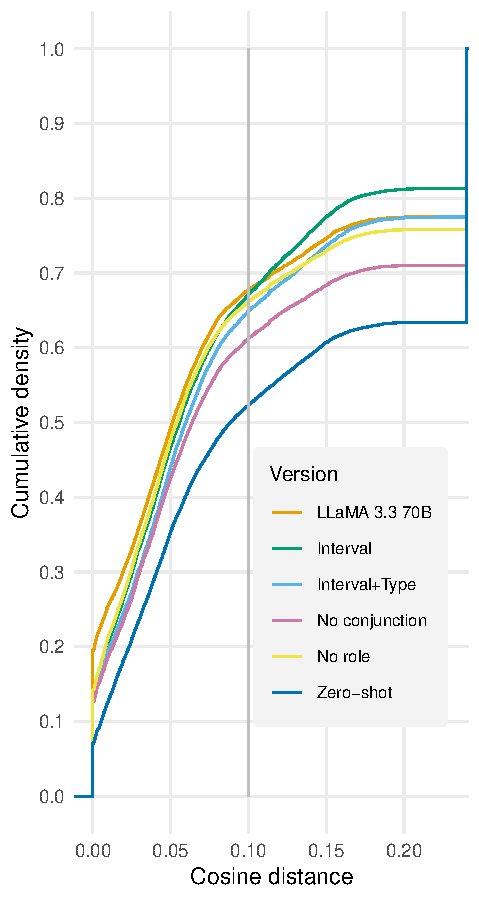
\includegraphics[page=1, width=\linewidth]{Chapters/chapter-05/images/Plots_tables/prompt_ablation_updated_figure.pdf}
    \end{minipage}
    \hfill
    \begin{minipage}[t]{0.242\textwidth}
    \centering
    \includegraphics[page=2, width=\linewidth]{Chapters/chapter-05/images/Plots_tables/prompt_ablation_updated_figure.pdf}
    \end{minipage}
    \hfill
    \begin{minipage}[t]{0.242\textwidth}
    \centering
    \includegraphics[page=3, width=\linewidth]{Chapters/chapter-05/images/Plots_tables/prompt_ablation_updated_figure.pdf}
    \end{minipage}
    \hfill
    \begin{minipage}[t]{0.242\textwidth}
    \centering
    \includegraphics[page=4, width=\linewidth]{Chapters/chapter-05/images/Plots_tables/prompt_ablation_updated_figure.pdf}
    \end{minipage}
    
    
    

\end{ChFiveFloatBody}
\caption{Comparison of \texttt{Llama 3.3 70B} prompt ablation and variant methods for extracting temporal clinical events from case reports. From left to right: (\textbf{A}) event match cumulative distribution function, (\textbf{B}) concordance box plots, (\textbf{C}) time discrepancy from manual annotation timestamps among matched events (overall), and (\textbf{D}) time discrepancy disaggregated by clinician annotator timestamp (time from presentation).}\ChFiveFloatLabel{ch05:fig:prompt_ablation}
\end{figure}














